%
% File acl2021.tex
%
%% Based on the style files for EMNLP 2020, which were
%% Based on the style files for ACL 2020, which were
%% Based on the style files for ACL 2018, NAACL 2018/19, which were
%% Based on the style files for ACL-2015, with some improvements
%%  taken from the NAACL-2016 style
%% Based on the style files for ACL-2014, which were, in turn,
%% based on ACL-2013, ACL-2012, ACL-2011, ACL-2010, ACL-IJCNLP-2009,
%% EACL-2009, IJCNLP-2008...
%% Based on the style files for EACL 2006 by 
%%e.agirre@ehu.es or Sergi.Balari@uab.es
%% and that of ACL 08 by Joakim Nivre and Noah Smith

\documentclass[11pt,a4paper]{article}
\usepackage[hyperref]{acl2021}
\usepackage{times}
\usepackage{latexsym}
\renewcommand{\UrlFont}{\ttfamily\small}

% This is not strictly necessary, and may be commented out,
% but it will improve the layout of the manuscript,
% and will typically save some space.
\usepackage{microtype}
\usepackage{graphicx}

%\aclfinalcopy % Uncomment this line for the final submission
%\def\aclpaperid{***} %  Enter the acl Paper ID here

%\setlength\titlebox{5cm}
% You can expand the titlebox if you need extra space
% to show all the authors. Please do not make the titlebox
% smaller than 5cm (the original size); we will check this
% in the camera-ready version and ask you to change it back.

\newcommand\BibTeX{B\textsc{ib}\TeX}

% Standard package includes
\usepackage{times}
\usepackage{url}
\usepackage{latexsym}
\usepackage{graphicx}
\usepackage{xcolor}
\usepackage{longtable}
\usepackage{tikz}
\usetikzlibrary{calc}
\usepackage[draft]{todo}
\usepackage[normalem]{ulem}
\usepackage{xspace}
\usepackage{float}
\usepackage{amsmath,amsfonts,amssymb}
\usepackage{algorithm, algorithmic}

\usepackage{tikz}
\usepackage{pgfplots}
\usepackage{pgfplotstable}

\usepackage{soulutf8}
\usepackage{tabularx}

\usepackage{multirow}
\usepackage{adjustbox}
\usepackage{caption}
\usepackage{subcaption}

\newcommand{\fyTodo}[1]{\Todo[FY:]{\textcolor{orange}{#1}}}
\newcommand{\fyTodostar}[1]{\Todo*[FY:]{\textcolor{orange}{#1}}}
\newcommand{\fyDone}[1]{\done[FY]\Todo[FY:]{\textcolor{orange}{#1}}}
\newcommand{\fyFuture}[1]{\done[FY]\Todo[FY:]{\textcolor{red}{#1}}}
\newcommand{\fyDonestar}[1]{\done[FY]\Todo[FY:]{\textcolor{orange}{#1}}}
\newcommand{\revision}[1]{\textcolor{red}{#1}}
\newcommand{\revisiondel}[1]{}
\newcommand{\src}{\ensuremath{\mathbf{f}}} % source sentence
\newcommand{\trg}{\ensuremath{\mathbf{e}}} % target sentence
\newcommand{\domain}[1]{\texttt{\textsc{#1}}}
\newcommand{\system}[1]{\texttt{{#1}}}

\newcommand{\vlambda}{\ensuremath{\boldsymbol\lambda}\xspace} % parameters vector for a distribution
\newcommand{\vtheta}{\ensuremath{\boldsymbol\theta}\xspace} % parameters vector for a distribution
\newcommand{\vpsi}{\ensuremath{\boldsymbol\psi}\xspace} % parameters vector for a distribution
\newcommand{\indic}[1]{\ensuremath{\mathbb{I}(#1)}}
% \newcommand{\SB}[1]{\textcolor{green}{#1}}
% \newcommand{\SW}[1]{\textcolor{red}{#1}}
\newcommand{\SB}[1]{\textbf{#1}}
\newcommand{\SW}[1]{\underline{#1}}
% limits underneath
\DeclareMathOperator*{\argmin}{arg\,min}
\DeclareMathOperator*{\argmax}{arg\,max}
\renewcommand\textfraction{.1}
\renewcommand\floatpagefraction{.95}
\newcommand{\sbcl}[2]{{\scriptsize #1 \hfill $|$ \hfill  #2}}
\usepackage{multirow}
\usepackage{adjustbox}

\title{Improving Multi-Domain Neural Machine Translation with Differential Data Selection}

\author{First Author \\
  Affiliation / Address line 1 \\
  Affiliation / Address line 2 \\
  Affiliation / Address line 3 \\
  \texttt{email@domain} \\\And
  Second Author \\
  Affiliation / Address line 1 \\
  Affiliation / Address line 2 \\
  Affiliation / Address line 3 \\
  \texttt{email@domain} \\}

\date{}

\begin{document}
\maketitle
\begin{abstract}
  When building machine translation systems, one often needs to make the best out of heterogeneous sets of parallel data in training to achieve the best test performance in one or several domain(s) of interest. This multi-source / multi-domain adaptation problem is often approached with instance selection or reweighting strategies, most of which pre-suppose an ex-ante assessment of the relevance of training instances. In this paper, we study the recently proposed Differential Data Selection (DDS) model and explore its ability to serve as a generic framework for these various situations. Our experiments study both domain adaptation and multi-domain learning and show that DDS often enables to outperform more heuristic adaptation strategies. We also introduce variants that boosts DDS performance of adapter-based multi-domain systems.\fyTodo{Keep this part ?}
%   This is a well-known issue, which has given raise to a rich litterature in under the umbrellas of domain adaptation or multi-domain 

%   The priority of the in-domain performance in the overall evaluation affects the choice of choosing data. The problem falls in the data selection category in the domain adaptation topic. Several data selection methods pre-compute the domain-relatedness of training examples and use these scores to build mini-batches in the training while other works propose dynamic strategies to build training mini-batches based on reinforcement learning.
% In this study, we first formulate the most general algorithm for training the Neural Machine Translation (NMT) model given a predefined priority of the domains. Then, we apply a recently proposed method to solve the problem. We also report a disadvantage of DDS and fix it by proposing a minor development for DDS. Our experiments with a large sample of multi-domain systems show several important benefits of DDS in multi-domain NMT.
\end{abstract}

\section{Introduction}\label{sec:intro}
A typical setting in machine translation (MT) is to collect the largest possible collection of parallel data for the chosen language pair, with the intent to achieve optimal performance for a task of interest. In such situations, the training data distribution is opportunistic, while the test data distribution is chosen and fixed; a key component in training is then to mitigate the detrimental effects of a possible mismatch between these distributions. Single-source and multi-source domain adaptation (DA) is a well-studied instance of this setting (see \cite{Chu2017comparison} for a review) , and so is multi-domain (MD) learning \cite{Chu18multilingual,Zeng18multidomain,Jiang19multidomain,Pham21revisiting}. A related situation is multilingual machine translation \cite{Firat16multiway,Ha16towards,Johnson17google,Arivazhagan19massively}\fyTodo{Add more recent work}, where the heterogeneity of training data not only corresponds to variations in topic, genre or register, but also in language.

\fyTodo{Label or covariate shift ?}
This problem is often approached with \emph{static} instance selection or re-weighting strategies, where the available training data is used in proportion to its relevance for the chosen test conditions. Finding the optimal balance of training data is however a challenging task due, for instance, to similarity between domains / languages, but also due to regularization effects of out-of-domain data; it may also be suboptimal, as some target domains or languages might be easier to train than others. Several recent proposals \cite{Wang17instance,Kumar19reinforcement,Wang20learning-multi} have explored ways to instead consider \emph{dynamic} data selection strategies. We study in this contribution the proposal of \citet{Wang20balancing}, initially introduced for multilingual MT, with the goal to evaluate its potential in various single-domain and multi-domain adaptation settings and assess DDS, both in its basic version and with our improvements, as an effective replacement to standard heuristics approaches.

Based on experimental results obtained on a diverse set of domains, our main conclusions are that (a) using DDS often yields overall performance that are as good as the standard fine-tuning strategy for domain adaptation; (b) DDS can effectively handle a variety of test target distributions without any meta-parameter search; (c) our extension of DDS is able to boost its performance when used in conjunction to the adapter model of \citet{Bapna19simple}.

% one often needs to make the best out of heterogeneous sets of parallel data in training to achieve the best test performance in one or several domain(s) of interest. This multi-source (multi-domain) adaptation problem is often approached with instance selection or reweighting strategies, most of which pre-supposes an ad-hoc assessment of relevance for training sentences. In this contribution, we study the recently proposed Differential Data Selection (DDS) model  and explore its ability to serve an effective generic framework for these various situations. Our experiments for both domain adaptation and multi-domain learning show that DDS often enables to outperform heuristic training strategies; we also introduce a variant that boosts DDS performance of adapter-based multi-domain systems.

\section{Learning with multiple data sources} \label{sec:mdmt}

We conventionally define a domain $d$ as a distribution $\mathcal{D}_d(x)$ over some feature space $\mathcal{X}$ that is shared across domains \citep{Pan10asurvey}: in machine translation, $\mathcal{X}$ is the representation space for input sentences; each domain corresponds to a specific source of data, and may differ from the other data sources in terms of textual genre, thematic content \cite{Chen16guided,Zhang16topicinformed}, register \cite{Sennrich16politeness}, style \cite{Niu18multitask}, etc. Translation in domain $d$ is formalized by a translation function $h_d(y|x)$ pairing sentences in a source language with sentences in a target language $y \in \mathcal{Y}$. $h_d$ is usually assumed to be deterministic (hence $y = h_d(x)$), but might differ from one domain to the other.

It is usual in MT to opportunistically collect training samples from several domains, which means that training instances are distributed according to the mixture $\mathcal{D}^s$ such that $\mathcal{D}^s(x) = \sum_{d=1}^{n_d} \lambda^{s}(d) \mathcal{D}_d(x)$, where $\{\lambda^{s}(d), d=1 \dots n_d\}$ are the corresponding mixture weights satisfying $\sum_d \lambda^{s}(d)=1$.

The main challenge is then to make the best of this heterogeneous data, with the aim to achieve the optimal performance for the intended test conditions. These might correspond to data from just one of the training domains, as in standard supervised (multi-source) domain adaptation; a more difficult case is when the test data is from one domain unseen in training (unsupervised domain adaptation); in multi-domain adaptation finally the test distribution is itself a mixture of domains, some of which may also be observed in training.  Without loss of generality, one may then assume that the test distribution takes the form $\mathcal{D}^{t}(x) = \sum_d \lambda^{t}(d) \mathcal{D}_d(x)$ - with only one non-null  component in the case of fine-tuning.
These situations are illustrated in Figure~\ref{fig:mdmt-lambdas}.
\begin{figure}[h]
  \centering
  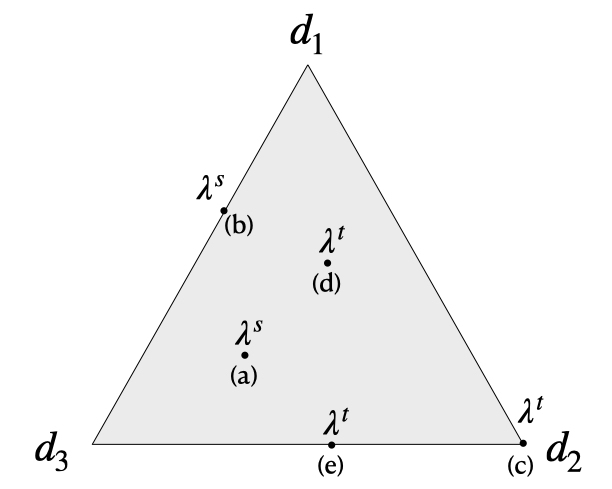
\includegraphics[width=0.48\textwidth]{mdmt-lambdas}
  \caption{Training and testing with distribution mismatch. We consider just three domains, and represent vectors of mixture weights $\vlambda^{s}$ and $\vlambda^{t}$ in the 3-dimensional simplex. Training with weights in (a) and testing with weights in (c) is supervised multi-source domain adaptation to domain~2 ($d_2$), while (b)-(c) is the unsupervised version, with no training data from $d_2$; training with weights in (a) and testing with weights in (d) is multi-domain learning, also illustrated with configurations (a)-(e) (training domain $d_1$ is not seen in test), and (b)-(d)  (test domain $d_2$ is unseen in training).}\label{fig:mdmt-lambdas}
\end{figure}

These situations have been amply documented from a theoretical perspective (eg.\ \cite{Mansour09multiple,Mansour09domainadaptation,Hoffman18algorithms}). A general recommandation in the DA setting  is to adjust the sampling distribution used to optimize the system so as to compensate for the mismatch between $\mathcal{D}^s(x)$ and $\mathcal{D}^t(x)$. This can be approximated by reweighting instances, or more conveniently domains, which are selected during training with a probability $\lambda^{l}(d)$, with $\lambda^{l}(d) \neq \lambda^{s}(d)$.

A more practical standard approach to supervised DA is \emph{fine-tuning} \cite{Luong15stanford,Freitag16fast}, where $\vlambda^{l}$ is allowed to vary during the course of learning. With our notations, this approach amounts to first learning an initial parameter value with all the data ($\forall d, \lambda^{l}(d) = \lambda^{s}(d)$), then to continue training with only batches from the test domain $d_t$ ($\lambda^{l}(d) = \indic{d = d_t}$) with $\indic{A}$ the indicator function for predicate $A$. Note that this strategy is potentially suboptimal, as some out-of-domain samples may contribute to the final performance due to eg.\ domain overlap. Optimizing the learning distribution in multi-domain settings is even more challenging, as the learner has to best take advantage of potential domains overlaps, and also of the fact that some domains might be easier to learn than others.\fyTodo{How to measure this?} 

Differentiable data selection (DDS), proposed by \citet{Wang20optimizing} and later applied to multilingual machine translation by \citet{Wang20balancing}, introduces an additional degree of freedom and allows to iteratively learn an optimal value for $\lambda^{l}$, as we now explain.

% === The part on multidomain training has been moved to the end.

\section{Differential Data Selection} \label{sec:dds}
\subsection{Basic principles}
Assuming training data from $n_d$ domains $d_1 \dots d_{n_d}$, we denote the size of the training corpus from domain $d$ as  $N^{s}_d$, and $N^{s} = \sum_d N^{s}_d$ is the total number of training samples. We use $\widehat{\mathcal{D}^l_d}$ and $\widehat{\mathcal{D}^t _d}$ to denote the empirical train and test distributions for domain $d$, and \revision{$\widehat{\mathcal{D}^{u}}(x;\lambda^{u}) = \sum_{d} \lambda^{u}(d) \widehat{\mathcal{D}^{u}_d}(x)$ for $u\in\{l,t\}$} \fyTodo{$\widehat{\mathcal{D}}(x;\lambda) = \sum_{d} \lambda(d) \widehat{\mathcal{D}_d}(x)$}. In our setting,  $\vlambda^t$, and hence $\widehat{\mathcal{D}^t}(x;\vlambda^t)$ are fixed and predefined, approximated with an equivalent number of development corpora. Training optimizes the parameters $\vtheta$ of a neural translation model.

Sampling training domains using a distribution $\lambda^{l}$ results in a parameter estimate $\theta(\lambda^{l})$, delivering performance that can be estimated on the development set using $\lambda^{t}$. \citet{Wang20optimizing,Wang20balancing} then formulate the problem of finding an optimal sampling strategy $\lambda^{l}_{*}$ maximizing performance on the development data as the following bi-level optimization problem:
\begin{equation} \label{eq:bilevel}
\begin{split}
\vlambda^{l}_* &= \displaystyle{\mathop{\argmin}_{\lambda^{l}} J(\theta^*(\vlambda^{l}), \vlambda^{t})} \\
					& \theta^*(\vlambda^{l}) = \displaystyle{\mathop{\argmin_{\vtheta}} J(\vtheta, \vlambda^{l})}, 
\end{split}
\end{equation}
where we use the following notations:% \fyTodo{Overload Q, from domain to instances to pairs}

\begin{align*}
J(\vtheta, \vlambda^{t} ) &= \displaystyle{\mathop{\sum}_{(x,y) \sim \widehat{\mathcal{D}^{t}(x)}} \ell(\vtheta,x,y)} \\
J(\vtheta, \vlambda^{l}) &= \displaystyle{\mathop{E_{(x,y) \sim \widehat{\mathcal{D}^{l}(x)}}[\ell(\vtheta,x,y)]}} \\
l(\vtheta,x,y) &= - log P(x,y;\vtheta)
\end{align*}
Problem~\eqref{eq:bilevel} can be approached by coordinate gradient descent alternating between $\lambda^{l}$ and $\vtheta$. \citet{Wang20balancing} limit the search space of $\vlambda^{l}$ to a parameterized differentiable function $\vlambda^{l}(\vpsi)$. Given $\vpsi_t$ at time step $t$, $\vtheta_t$ is updated via usual gradient descent as follows:
\begin{align*}
\vtheta_{t+1} &= \vtheta_t - \mathbf{lr}_{nmt} * \frac{\partial l(\vtheta_t, x,y)}{\partial \vtheta} \\
x,y &\sim \widehat{\mathcal{D}^l}(x;\vlambda^l(\psi_t)) = \displaystyle{\mathop{\sum}_{d=1}^K} \lambda^l(d;\psi_t) * \widehat{D_d}(x) \\
\end{align*}
Given $\vtheta_t$, $\psi_t$ is updated via the Reinforce algorithm \cite{Williams92reinforce}:\fyTodo{Rewrite this correctly with domain average reward}
%\begin{align*}
%  \psi_{t+1} &= \psi_t + \mathbf{lr}_{data} * R(x,y) * \\
%  & \quad\quad \frac{\partial log(\lambda^l(\psi_t)(x,y))}{\partial \psi} \\
%x,y &\sim \lambda^l (\psi_t) \\
%R(x,y) &= \langle \frac{\partial l(\theta',x,y)}{\partial \theta}, \frac{\partial J(\theta_{t+1}, \lambda^l)}{\partial \theta} \rangle \\
%\theta' &= \theta_t - \mathbf{lr}_{nmt} * \frac{\partial l(\theta_t, x,y)}{\partial \theta} \\
%\end{align*}

\begin{align*}
\psi_{t+1} &= \psi_t + \mathbf{lr}_{data} * \displaystyle{\mathop{\sum}_{d=1}^K} R(d) * \frac{\partial log(\lambda^l(\psi_t)(d))}{\partial \psi} \\
  R(d) &= E_{x,y \sim \widehat{D_d}}[\langle \frac{\partial l(\theta_t,x,y)}{\partial \theta}, \frac{\partial J(\theta', \lambda^t)}{\partial \theta} \rangle] \\
  \theta' &= \theta_t - \mathbf{lr}_{nmt} * \frac{\partial l(\theta_t, x,y)}{\partial \theta} \\
\end{align*}

$\mathbf{lr}_{data}$ is the learning rate of the parameter of the sampler. $\mathbf{lr}_{nmt}$ is the learning rate of the parameter of the NMT system. \fyTodo{Explain lr, may be more}\fyTodo{More refs to the algorithm }
% To apply this method to multi-domain training (\system{Multi-DDS}), we limit the search family of training distribution $D_{trn}$ to the family of mixture of K in-domain training distribution such as $\sum_d \lambda^{s}_{d} \mathcal{D}_d(x,y)$. We also parameterize $\lambda^{s}_{d}$ using Softmax function so that $\lambda^{s}_{d} = \text{Softmax}(\psi)_d$ where $\psi \in \mathbb{R}^K$.
\subsection{DDS for (multi) domain adaptation}

This setting is pretty general and can in principle accomodate the variety of situations mentioned  above, and many more: basic domain adaption, multi-domain adaptation with various target distributions, possibly including domains unseen in training. In our experiments we would like to better assess the actual potential of DDS is these settings and seek to experimentally answer the following questions:
\begin{itemize}
\item is DDS a viable alternative to conventional fine-tuning? In particular does it enable to better take advantage of relevant data from other domains?
\item is DDS also a viable option in multidomain adaptation scenarios?
\item does DDS also enable to perform unsupervised (multi-) domain adaptation?\fyTodo{TBContinued}
\end{itemize}

These questions are further discussed in Section~\ref{sec:results}. We now turn to our experimental conditions.

\section{Experimental settings} \label{sec:exp}

\subsection{Data and metrics \label{ssec:corpora}}
We experiment with translation from English into French and use texts initially originating from 6~domains, corresponding to the following data sources: the UFAL Medical corpus V1.0 (\domain{med})\footnote{\url{https://ufal.mff.cuni.cz/ufal_medical_corpus}.\revision{We only use the in-domain (medical) subcorpora: PATR, EMEA, CESTA, ECDC.}}; the European Central Bank corpus (\domain{bank}) \cite{Tiedemann12parallel}; the JRC-Acquis Communautaire corpus (\domain{law}) \cite{Steinberger06acquis}; documentations for KDE, Ubuntu, GNOME and PHP from the Opus collection \cite{Tiedemann09news}, merged in a \domain{it}-domain; TedTalks (\domain{talk}) \cite{Cettolo12wit}, and the Koran (\domain{rel}). Complementary experiments also use v12 of the News Commentary corpus (\domain{news}). Most corpora are available from the Opus website.\footnote{\url{http://opus.nlpl.eu}} These corpora were deduplicated and tokenized with in-house tools; statistics are in Table~\ref{tab:Corpora}. To reduce the number of types and build open-vocabulary systems, we use Byte-Pair Encoding \cite{Sennrich16BPE} with 30,000 merge operations on a corpus containing all sentences in both languages.\fyDone{Add \# number of tokens, also specificity ?}%

We randomly select in each corpus a development and a test set of 1,000 lines and keep the rest for training. Validation sets are used to chose the best model according to the average BLEU score \cite{Papineni02bleu}.\footnote{We use truecasing and the \texttt{multibleu} script.}\fyDone{A word about meta-parameter settings} Significance testing is performed using bootstrap resampling \cite{Koehn04statistical}, implemented in compare-mt\footnote{\url{https://github.com/neulab/compare-mt}} \cite{Neubig19compare-mt}. We report significant differences at the level of $p=0.05$.\fyDone{Fix correct p value}

%for contrast experiments, we also use supplementary test sets from three other domains: the official Khresmoi testset \cite{Khresmoi17test}, which is close to EMEA, News test 2014 \cite{Bojar14findings}, and IWSLT 2010 (Talk track) \cite{Paul10overview}. This enables us to evaluate the loss in performance when the test set is from a domain not seen in training.
% The model is also required to achieve comparable performance to generic model. To do so, we use newstest 2009 and IWSLT 2010 whose contain does not particularly belong to any domain.

\begin{table*}[htbp]
  \centering
  \begin{tabular}{|l|ccccccc|} %*{4}{|r|}}
    \cline{2-8} 
    %\multicolumn{4}{|l|}{Vocab size - En: 30,165, Fr: 30,398}\\
    \multicolumn{1}{c|}{} & \multicolumn{1}{c}{\domain{med}} & \multicolumn{1}{c}{\domain{law}} & \multicolumn{1}{c}{\domain{bank}} & \multicolumn{1}{c}{\domain{it}} & \multicolumn{1}{c}{\domain{talk}} & \multicolumn{1}{c}{\domain{rel}} & \multicolumn{1}{c|}{\domain{news}} \\
    \hline 
    \# lines & 2609 (0.68) & 501 (0.13) & 190 (0.05) & 270 (0.07) & 160 (0.04) & 130 (0.03) & 260 (0) \\
    \# \revision{tokens}  &  133 / 154  &  17.1 / 19.6 &  6.3 / 7.3 &  3.6 / 4.6 &  3.6 / 4.0 &  3.2 / 3.4 & 7.8 / 9.2   \\
    \# \revision{types}  & 771 / 720 & 52.7 / 63.1 & 92.3 / 94.7 & 75.8 / 91.4 & 61.5 / 73.3 & 22.4 / 10.5 & - \\
    \# \revision{uniq} & 700 / 640 & 20.2 / 23.7 & 42.9 / 40.1 & 44.7 / 55.7 & 20.7 / 25.6 & 7.1 / 2.1 & - \\
    \hline
  \end{tabular}
  \caption{Corpora statistics: number of parallel lines ($\times 10^3$) and proportion in the training domain mixture (which does not contain \domain{news}), number English and French tokens ($\times 10^6$), number English and French types ($\times 10^3$), number of types that only appear in a given domain ($\times 10^3$). \domain{med} is the largest domain, containing almost 70\% of the sentences, while \domain{rel} is the smallest, with only 3\% of the data.
  }
\label{tab:Corpora}
\end{table*}

\fyTodo{Keep this ?}
We measure the distance between domains using the $\mathcal{H}$-Divergence \cite{Ben-David09atheory}, which relates domain similarity to the test error of a domain discriminator: the larger the error, the closer the domains.
%Formally, given test sets of size $m$ for domains $A$ and $B$, and $h(x)$ a trained domain predictor, $\mathcal{H}(A,B)$ is computed %as:
%$$
%\mathcal{H}(A,B) = 2(1 - [\frac{1}{m} \sum_{x:h(x) = B} \mathbb{I}( x \in A) + \frac{1}{m} \sum_{x: h(x) = A} \mathbb{I}(x \in B)]),
% $$
% where $\mathbb{I}$ is the indicator function.
Our discriminator is a SVM independently trained for each pair of domains, with sentence representations derived via mean pooling from the source side representation of the generic Transformer model. We used the scikit-learn\footnote{\url{https://scikit-learn.org}} implementation with default values.\fyDone{Inform the classifier details}\fyDone{Insert tableau} Results in Table~\ref{tab:domaindist} show that all domains are well separated from all others, with \domain{rel} being the furthest apart, while \domain{talk} is slightly more central.

\begin{table}\centering
  \begin{tabular}{|l*{5}{|r}|} 
  \cline{2-6}
  \multicolumn{1}{c|}{} & \domain{law} & \domain{bank} & \domain{talk} & \domain{IT} & \domain{rel} \\ \hline
    \domain{med} &1.93 &1.97 &1.9 &1.93 &1.97 \\
    \domain{law}   && 1.94 & 1.97 &1.93 & 1.99 \\
    \domain{bank} &&&1.98 &1.94 &1.99 \\
    \domain{talk}   &&&&1.92 &1.93 \\
     \domain{IT}     &&&&& 1.99 \\ \hline
  \end{tabular}
  \caption{The $\mathcal{H}$-divergence between domains}
  \label{tab:domaindist}
\end{table}

\subsection{Baseline architectures \label{ssec:baseline}}
Our baselines are standard for multi-domain systems.\footnote{We however omit domain-specific systems trained only with the corresponding subset of the data, which are always inferior to the mix-domain strategy \cite{Britz17mixing}.} Using Transformers \cite{Vaswani17attention} implemented in OpenNMT-tf\footnote{\url{https://github.com/OpenNMT/OpenNMT-tf}} \cite{Klein17opennmt}, we build the following systems:

\begin{itemize}
\itemsep0em 
\item Generic models trained with various predefined mixtures of the training data taking the form:
\begin{align} \label{mixture:trn}
\lambda_{\alpha}(d) = \frac{q_d^{\alpha}}{\displaystyle{\mathop{\sum}_{d=1}^{n_d}q_d^{\alpha}}} &&
q_d = \frac{\mid N^{s}_d \mid}{\displaystyle{N^{s}}} % \mathop{\sum}_{i=1}^K\mid D_i \mid}}
\end{align} 
with $\alpha \in [0,0.25,0.5,0.75,1.0]$. These systems are denoted \system{Mixed-$\alpha$} below. \system{Mixed-$0$} uses a uniform domain distribution, \system{Mixed-$1.0$} simple uses the observed domain distribution.
%on a concatenation of all corpora (\texttt{Mixed}). We develop two versions\footnote{In fact three: to enable a fair comparison with WDCMT, a RNN-based variant is also trained and evaluated. \revision{This system appears as \system{Mixed-Nat-RNN} in Table~\ref{tab:performance}}.} of this system, one where the domain unbalance reflects the distribution of our training data \revision{given in Table~\ref{tab:Corpora}} (\system{Mixed-Nat}) and one where all domains are equally represented in training (\system{Mixed-Bal}). The former is the best option when the train mixture $\mathcal{D}^s$ is also expected in testing; the latter should be used when the test distribution is uniform across domains. Accordingly, we report two aggregate scores: a weighted average reflecting the training distribution, and an unweighted average, meaning that test domains are equally important.
\item fine-tuned models \cite{Luong15stanford,Freitag16fast}, based on the \system{Mixed-$1.0$} system, further trained on each domain for at most 20~000 iterations, with early stopping when the dev BLEU stops increasing. The full fine-tuning (\system{FT-Full}) procedure may update all the parameters of the initial generic model, resulting in six systems each adapted for one domain, with no parameter sharing across domains.

\item two multi-domain versions of the approach of \newcite{Bapna19simple}, denoted \system{FT-Res} and \system{MDL-Res}, where a domain-specific adaptation module is added to all the Transformer layers; within each layer, residual connections enable to short-cut this adapter. The former variant corresponds to the original proposal of \citet{Bapna19simple} (see also \cite{Sharaf20metalearning}). It fine-tunes the adapter modules of a \system{Mixed-$1.0$} system independently for each domain, keeping all the other parameters frozen. The latter uses the same architecture, but a different training procedure and learns all parameters jointly from scratch with the prefixed mixtures of training data \ref{mixture:trn}.\fyTodo{Keep this ?}
  
\item Our comparison of multi-domain systems includes baselines with fixed data mixtures corresponding to $\vlambda_0$ and $\vlambda_1$, and our own reimplementations of recent proposals from the literature:\footnote{\revision{Further implementation details are in supplementary material.}}\fyTodo{Choose a reasonnable MD baseline }

\end{itemize}

All models use embeddings and hidden layers sizes of dimension~512. Transformer models contain 8~attention heads in each of the 6+6 layers; the inner feedforward layer contains 2048 cells. The adapter-based systems (see below) additionally use an adaptation block in each layer, composed of a 2-layer perceptron, with an inner $\operatorname{ReLU}$ activation function operating on normalized entries of dimension~1024. 
Training uses batches of~12,288 tokens, Adam with parameters $\beta_1=0.9$, $\beta_2= 0.98$, Noam decay ($warmup\_steps=4000$), and a dropout rate of $0.1$ in all layers.

\subsection{DDS-based systems } \label{ssec:dds-sys}

The architecture of DDS based-systems is identical to that of our baselines, and only differ in the training regime. Their behavior only depends on (a) the initial domain distribution at the start of training $\vlambda^{l}_{t=0}$, and (b) the targeted (dev/test) distribution $\vlambda^{t}$. We will thus report these systems as \system{DDS($\vlambda^{l}_{t=0}$, $\vlambda^{t}$)}. The domain distribution attained at the end of training will be denoted  $\vlambda^{l}_{*}$.

\section{Results and discussion \label{sec:results}}

\subsection{DDS for single-domain and multi-domain adapation}

\subsubsection{Fine-tuning experiments}

\fyTodo{Fix the table}
In Table~\ref{tab:finetuning}, we compare the results of fine-tuning a system initially trained with a uniform mixture\fyTodo{uniform or natural?} of domains with the result of learning from scratch, also with a initial uniform distribution. \fyTodo{What do we see ? How about domain proximity ? - show a graph}. Note that the DDS systems are somewhat quicker to build, as we only train for 100K iterations (instead of 100K + 50K for the fine-tuning part).

\begin{table*}
  \centering \small
  \begin{tabular}{|l|*8{r|}} \hline
    domain \hfill $d=$ & \multicolumn{1}{c|}{\domain{ med}} & \multicolumn{1}{c|}{\domain{ law}} & \multicolumn{1}{c|}{\domain{bank}} & \multicolumn{1}{c|}{\domain{talk}} & \multicolumn{1}{c|}{\domain{ it }} & \multicolumn{1}{c|}{\domain{ rel}} & \multicolumn{1}{c|}{mean} \\ \hline
    Full-FT($d$) & \\
    \system{DDS($\vlambda_0, \indic{d}$)} & \\
    \% & \\ \hline
    \system{DDS($\vlambda_0, \indic{d}$)} &  \\ \hline
    \% & \\ \hline\hline
    % Multidomain
    \system{Mixed-0} & \\
    \system{Mixed-0.5} & \\
    \system{Mixed-1} & \\
    \system{FT-Res} & \\\hline
    \system{DDS($\vlambda_1, \vlambda_0$)} & \\
    $\operatorname{KL}(\vlambda_*^{l}, \vlambda_0$) & \\
     $ \mathcal{H}(\vlambda_*^{l})$ &  \\
    \system{DDS($\vlambda_0, \vlambda_0$)} & \\ \hline
  \end{tabular}
  \caption{Baseline results for DDS. In the top part, for each domain, we report the scores of DDS targeting solely this domain and compare with full-fine-tuning. We also compute the percentage of in-domain data in the resulting mixture and its entropy.}
  \label{tab:finetuning}
\end{table*}

A first observation is DDS only better than FT for \domain{rel}, and worse for \domain{med} and \domain{law}. There seem to be a connection with the domain size, as \domain{rel} is small and benefits from data from other domains, while the opposite effect is observed for the larger \domain{med} and \domain{law}. For the three other domains, we do not see any marked difference, which we view as a positive result.

If we now look at the multi-domain results (bottom part of Table~\ref{}), we see that DDS actually does better than the two baseline strategies, but is not as good as using a fixed distribution with a well-chosen $\alpha$....\fyTodo{To be continued}

% \begin{table*}
%   \centering% \small
%   \begin{adjustbox}{width=2\columnwidth,center}
%   \begin{tabular}{|p{2cm}|*{13}{r|}} \hline
%     \multirow{2}{*}{Training} & \multicolumn{6}{|c}{$\lambda^t_d$} & \multicolumn{6}{|c|}{BLEU} & \multirow{2}{*}{BLEU} \\ \cline{2-13}	
%   mixture & \multicolumn{1}{c|}{\domain{ med}} & \multicolumn{1}{c|}{\domain{ law}} & \multicolumn{1}{c|}{\domain{bank}} & \multicolumn{1}{c|}{\domain{talk}} & \multicolumn{1}{c|}{\domain{ it }} & \multicolumn{1}{c|}{\domain{ rel}} & \multicolumn{1}{c|}{\domain{ med}} & \multicolumn{1}{c|}{\domain{ law}} & \multicolumn{1}{c|}{\domain{bank}} & \multicolumn{1}{c|}{\domain{talk}} & \multicolumn{1}{c|}{\domain{ it }} & \multicolumn{1}{c|}{\domain{ rel}} & average \\
%     \hline
%   \system{FT-Full} & 1.0 &0.0 & 0.0 &0.0 &0.0 & 0.0 &37.45&51.26&45.47&31.62&37.55&65.22& \\
%   \system{FT-Res} & 1.0 &0.0 & 0.0 &0.0 &0.0 & 0.0 &35.26 &54.09 &52.49& 31.86& 44.94& 89.54& 51.36\\
%   \system{Multi-DDS} & 1.0 &0.0 & 0.0 &0.0 &0.0 & 0.0 &35.26 &54.09 &52.49& 31.86& 44.94& 89.54& 51.36\\
%   \system{FT-Full} & 0.0 &1.0 & 0.0 &0.0 &0.0 & 0.0 &35.92& 54.87& 52.55& 32.55& 44.98& 90.28& 51.86\\
%   \system{FT-Full} & 1.0 &0.0 & 0.0 &0.0 &0.0 & 0.0 &35.26 &54.09 &52.49& 31.86& 44.94& 89.54& 51.36\\
%   \system{Multi-DDS} & 0.0 &1.0 & 0.0 &0.0 &0.0 & 0.0 &35.92& 54.87& 52.55& 32.55& 44.98& 90.28& 51.86\\
%   \system{FT-Full} & 0.0 &0.0 & 1.0 &0.0 &0.0 & 0.0 &36.11& 55.37& 51.76& 33.52& 46.23& 89.99& 52.16\\
%   \system{FT-Full} & 1.0 &0.0 & 0.0 &0.0 &0.0 & 0.0 &35.26 &54.09 &52.49& 31.86& 44.94& 89.54& 51.36\\
%   \system{Multi-DDS} & 0.0 &0.0 & 1.0 &0.0 &0.0 & 0.0 &36.11& 55.37& 51.76& 33.52& 46.23& 89.99& 52.16\\
%   \system{FT-Full} & 0.0 &0.0 & 0.0 &1.0 &0.0 & 0.0 &36.53&	55.03& 51.15& 33.98& 44.28& 87.22& 51.365\\
%   \system{FT-Full} & 1.0 &0.0 & 0.0 &0.0 &0.0 & 0.0 &35.26 &54.09 &52.49& 31.86& 44.94& 89.54& 51.36\\
%   \system{Multi-DDS} & 0.0 &0.0 & 0.0 &1.0 &0.0 & 0.0 &36.53&	55.03& 51.15& 33.98& 44.28& 87.22& 51.365\\
%   \system{FT-Full} & 0.0 &0.0 & 0.0 &0.0 &1.0 & 0.0 &37.33& 54.56& 50.05& 33.47& 43.23& 77.51& 49.36\\
%   \system{FT-Full} & 1.0 &0.0 & 0.0 &0.0 &0.0 & 0.0 &35.26 &54.09 &52.49& 31.86& 44.94& 89.54& 51.36\\
%   \system{Multi-DDS} & 0.0 &0.0 & 0.0 &0.0 &1.0 & 0.0 &37.33& 54.56& 50.05& 33.47& 43.23& 77.51& 49.36\\
%   \system{FT-Full} & 0.0 &0.0 & 0.0 &0.0 &0.0 & 1.0 &37.33& 54.56& 50.05& 33.47& 43.23& 77.51& 49.36\\
%   \system{FT-Full} & 1.0 &0.0 & 0.0 &0.0 &0.0 & 0.0 &35.26 &54.09 &52.49& 31.86& 44.94& 89.54& 51.36\\
%   \system{Multi-DDS} & 0.0 &0.0 & 0.0 &0.0 &0.0 & 1.0 &37.33& 54.56& 50.05& 33.47& 43.23& 77.51& 49.36\\
%   \hline
%   \end{tabular}
%   \end{adjustbox}
%   \label{tab:redomains}
% \end{table*}

\begin{table*}[htb]
  \centering% \small
  \begin{adjustbox}{width=1.0\textwidth,center}
  \begin{tabular}{|p{3.0cm}|*{13}{r|}} \hline
    \multirow{2}{*}{Name} & \multirow{2}{*}{$sim\_iter$} & \multirow{2}{*}{parameterization} & \multirow{2}{*}{entropy constraint} & \multicolumn{7}{|c|}{BLEU} \\ \cline{5-11}	
   & & & & \multicolumn{1}{c|}{\domain{ med}} & \multicolumn{1}{c|}{\domain{ law}} & \multicolumn{1}{c|}{\domain{bank}} & \multicolumn{1}{c|}{\domain{it}} & \multicolumn{1}{c|}{\domain{ rel }} & \multicolumn{1}{c|}{\domain{ talk}} & \multicolumn{1}{c|}{mean} \\
    \hline
  \system{$DDS\_FT (med)$} & 1 & softmax & no & 36.7&51.14&52&44.32&90.41&33.22&51.3\\
  \system{$DDS\_FT\_law$} & 1 & softmax & no &36.05&56.18&53.57&44.05&91.24&33.09&52.36\\
  \system{$DDS\_FT\_bank$} & 1 & softmax & no &36.15&54.17&54.29&41.33&89.95&31.54&51.24 \\
  \system{$DDS\_FT\_IT$} & 1 & softmax & no &34.39&48.98&52.82&46.8&85.3&31.37&49.94 \\
  \system{$DDS\_FT\_rel$} & 1 & softmax & no & 34.54&52.29&51.46&44.8&91.77&31.84&51.12\\
  \system{$DDS\_FT\_talk$} & 1 & softmax & no & 35.53&50.55&52.64&44.86&85.8&33.47&50.48\\
  \system{$FT\_full$} & NA & NA & NA & 37.74&59.21	&54.49&46.81&90.77&33.98&53.83\\
    \hline
    $\Delta$ & \\
  \end{tabular}
  \end{adjustbox}
  \caption{DDS as a fine-tuning recipe. We report scores with DDS and each target domain, and compare with full-fine-tuning. Note that the last line reports the results of 6 different fine tuning procedures.}
  \label{tab:finetuning-old}
\end{table*}\fyTodo{This table does not work- One line would be enough, where we compare autoFT with true FT}

\fyTodo{Works best for small domains ?}
\fyTodo{Curves for bank / medical ou law}
\fyTodo{Fine tune pour 2 domains ?}


\subsubsection{Multi-domain experiments}
Results for our multidomain experiments are in Table~\ref{tab:multidomains}.\fyTodo{Same table, line autoMD. We should be clear about the dev / test distribution - uniform ? so I would compare MIX with DDS(UNIF, UNIF) - DDS(NAT,UNIF) and not report / domain scores}

\begin{table*}
  \centering% \small
  \begin{adjustbox}{width=2\columnwidth,center}
  \begin{tabular}{|p{3.0cm}|*{13}{r|}} \hline
    \multirow{2}{*}{Training} & \multicolumn{6}{|c}{$\lambda^t_d$} & \multicolumn{6}{|c|}{BLEU} & \multirow{2}{*}{BLEU} \\ \cline{2-13}	
  mixture & \multicolumn{1}{c|}{\domain{ med}} & \multicolumn{1}{c|}{\domain{ law}} & \multicolumn{1}{c|}{\domain{bank}} & \multicolumn{1}{c|}{\domain{talk}} & \multicolumn{1}{c|}{\domain{ it }} & \multicolumn{1}{c|}{\domain{ rel}} & \multicolumn{1}{c|}{\domain{ med}} & \multicolumn{1}{c|}{\domain{ law}} & \multicolumn{1}{c|}{\domain{bank}} & \multicolumn{1}{c|}{\domain{talk}} & \multicolumn{1}{c|}{\domain{ it }} & \multicolumn{1}{c|}{\domain{ rel}} & average \\
    \hline
  \system{Mixed-$0.0$} & 0.166&0.166 &0.166 &0.166 &0.166 & 0.166 & 35.26 &54.09 &52.49& 31.86& 44.94& 89.54& 51.36\\
  \system{Mixed-$0.25$} & 0.166&0.166 &0.166 &0.166 &0.166 & 0.166 &35.92& 54.87& 52.55& 32.55& 44.98& 90.28& 51.86\\
  \system{Mixed-$0.5$} & 0.166&0.166 &0.166 &0.166 &0.166 & 0.166 &36.11& 55.37& 51.76& 33.52& 46.23& 89.99& 52.16\\
  \system{Mixed-$0.75$} & 0.166&0.166 &0.166 &0.166 &0.166 & 0.166 &36.53&	55.03& 51.15& 33.98& 44.28& 87.22& 51.365\\
  \system{Mixed-$1.0$} & 0.166&0.166 &0.166 &0.166 &0.166 & 0.166 &37.33& 54.56& 50.05& 33.47& 43.23& 77.51& 49.36\\
  \system{Multi-DDS} & 0.166&0.166 &0.166 &0.166 &0.166 & 0.166 & 37.26 & 55.07&50.96&33.49&43.41&90.76& 51.83 \\
  \system{Multi-DDS-v1} & 0.166&0.166 &0.166 &0.166 &0.166 & 0.166 & 36.96 & 55.55 & 52.88 & 33.06 & 44.52 &91.25 & 52.37\\
  \hline
  \end{tabular}
\end{adjustbox}
  \label{tab:multidomains}
\end{table*}

It is however striking to see that the distribution at the end of training is concentrated on few domains, and is quite remote from the targeted test distribution. Looking at the evolution of $\vlambda^l$ during training, we often observe a rich-get-richer effect, where a small number of domains manage to attract most of the samples, while others are almost completely ignored after a given number of iterations. This is illustrated on Figure~\ref{}, where we see....\fyTodo{Give illustration and numbers}

\subsection{Analysis}

\subsubsection{Winner-takes-all}
\cite{Wang20balancing} used a simple softmax function and the following parameterization of the sampler $\lambda^l(d;\psi) = \operatorname{softmax}(\psi)$ where $\psi \in \mathbb{R}^{n_d}$. This parameterization of the sampler will induce the following gradient:\fyTodo{Change name of obj. function}
\begin{align*}
\frac{\partial XXX}{\partial \psi_d} & = \displaystyle{\mathop{\sum}_{j=1}^{n_d}} R_j \frac{\partial \lambda^l(j; \psi)}{\partial \psi_d} \\
%	& = R_d \lambda^l(d; \psi)(1- \lambda^l(d; \psi)) - \displaystyle{\mathop{\sum}_{j\neq d}^{n_d}} R_j \lambda^l(d; \psi) \lambda^l(j; \psi)\\
	& = \lambda^l(d; \psi) (R_d- XXX)\\
\end{align*} 
The fact that the change of $\psi_d$ is proportional to $\lambda^l(d; \psi)$ can explain that the optimization often leads to a degenerate solution in which the sampler ignore almost domains except a few ones. In order to avoid the appearance of a ``rich-gets-richer'' effect and degenerate solutions such as Fig.~\ref{},

\begin{table*}
  \centering % \small
  \begin{adjustbox}{width=1.0\textwidth,center}
  \begin{tabular}{|p{2.0cm}|*{13}{r|}} \hline
    \multirow{2}{*}{Name} & \multirow{2}{*}{$sim\_iter$} & \multirow{2}{*}{parameterization} & \multirow{2}{*}{entropy constraint} & \multicolumn{6}{|c|}{BLEU} & \multirow{2}{*}{average} \\ \cline{5-10}	
   & & & & \multicolumn{1}{c|}{\domain{ med}} & \multicolumn{1}{c|}{\domain{ law}} & \multicolumn{1}{c|}{\domain{bank}} & \multicolumn{1}{c|}{\domain{talk}} & \multicolumn{1}{c|}{\domain{ it }} & \multicolumn{1}{c|}{\domain{ rel}} &  \\
    \hline
    \system{$config\_603$} & 1 & softmax & no & 37.26& 55.07& 50.96& 33.49& 43.41& 90.76& 51.83\\
    \system{$config\_616$} & 1 & softmax & yes & 36.96& 55.55& 52.88& 33.06& 44.52& 91.25& 52.37 \\
    \system{$config\_675$} & 10 & softmax & yes & 36.24& 55.67& 52.63& 32.74& 44.47& 90.45& 52.03\\
    \system{$config\_673$} & 10 & linear & yes & 36.02& 56.18& 52.96& 32.06& 45.2 & 90.94 & 52.23 \\
  \hline
  \end{tabular}
  \end{adjustbox}
  \caption{Controlling / regularizing the training distribution}
  \label{tab:performance}
\end{table*}

\begin{figure*}[htb]
\begin{subfigure}{.5\textwidth}
  \centering
  % include first image
  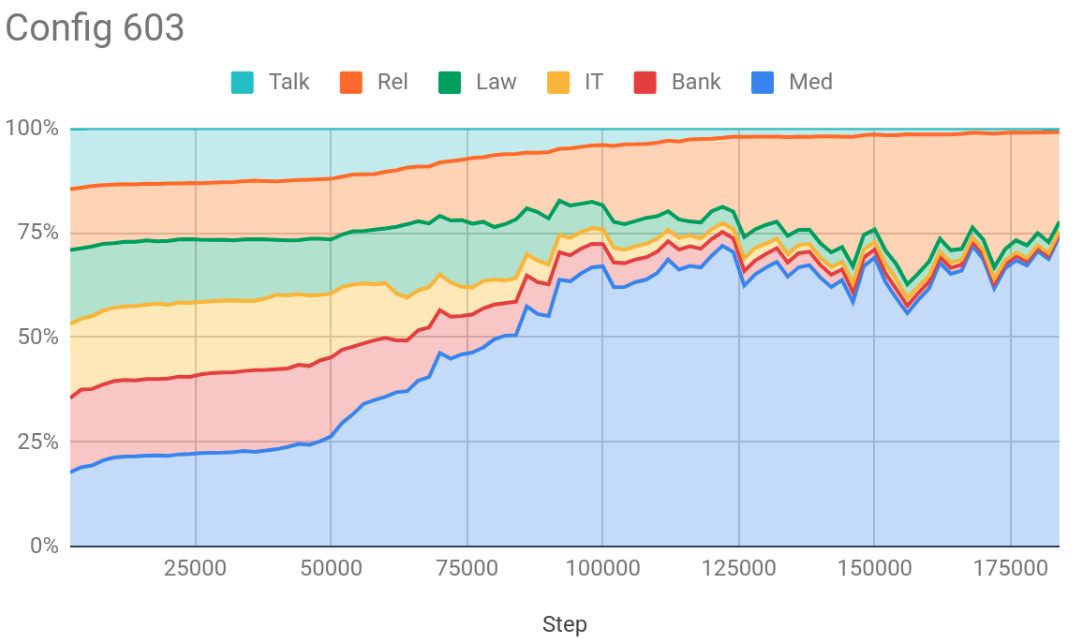
\includegraphics[width=.8\linewidth]{config603.png}  
  \caption{config 603}
  \label{fig:603}
\end{subfigure}
\begin{subfigure}{.5\textwidth}
  \centering
  % include second image
  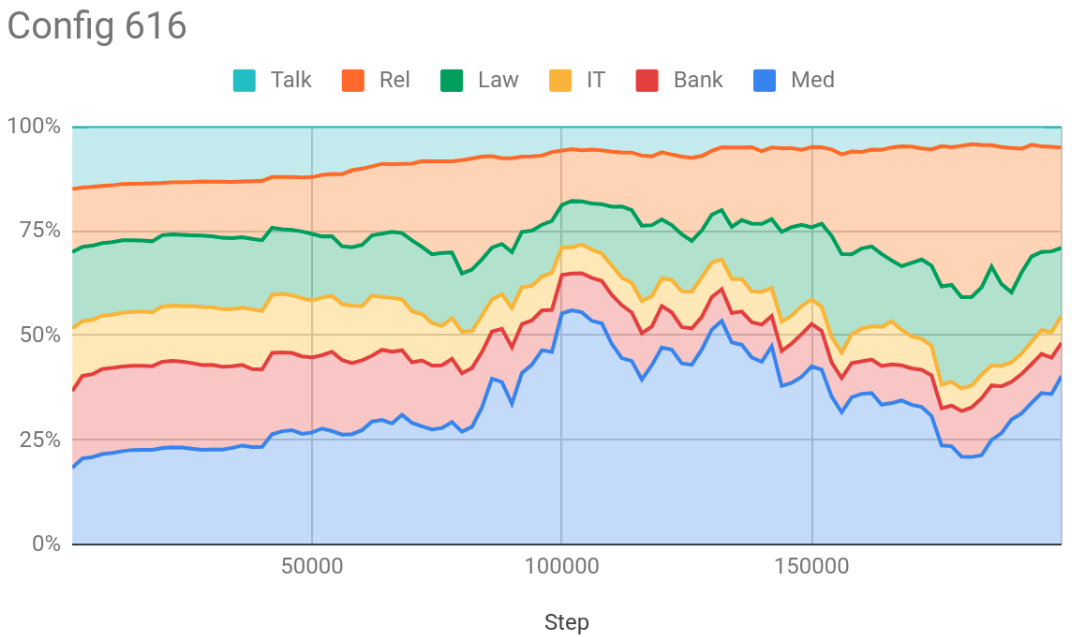
\includegraphics[width=.8\linewidth]{config616.png}  
  \caption{Config 616}
  \label{fig:616}
\end{subfigure}
\newline
\begin{subfigure}{.5\textwidth}
  \centering
  % include third image
  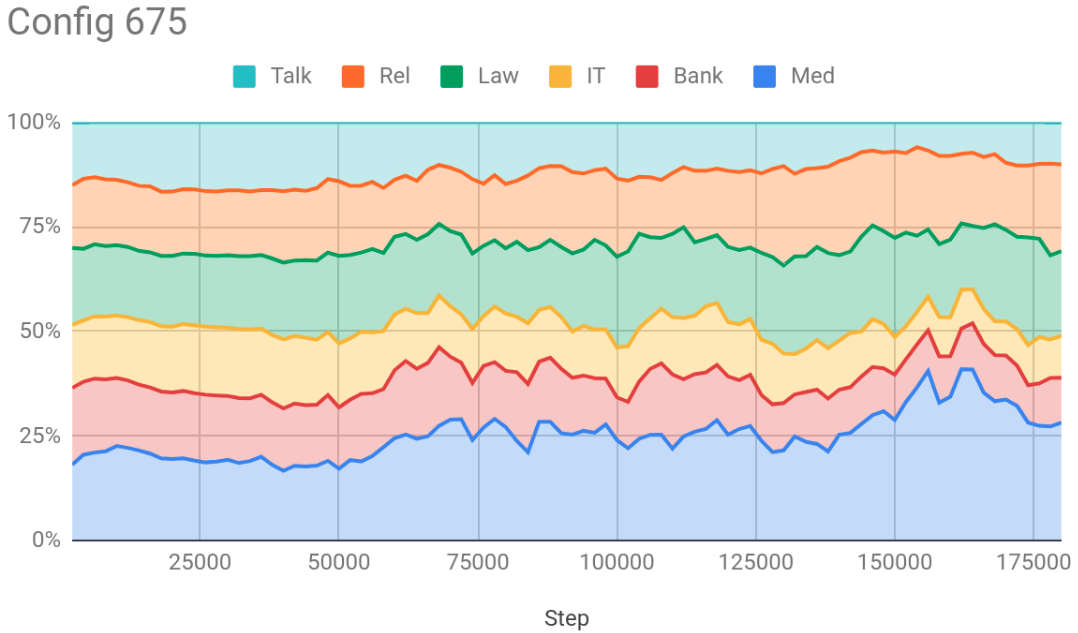
\includegraphics[width=.8\linewidth]{config675.png}  
  \caption{Config 675}
  \label{fig:675}
\end{subfigure}
\begin{subfigure}{.5\textwidth}
  \centering
  % include fourth image
  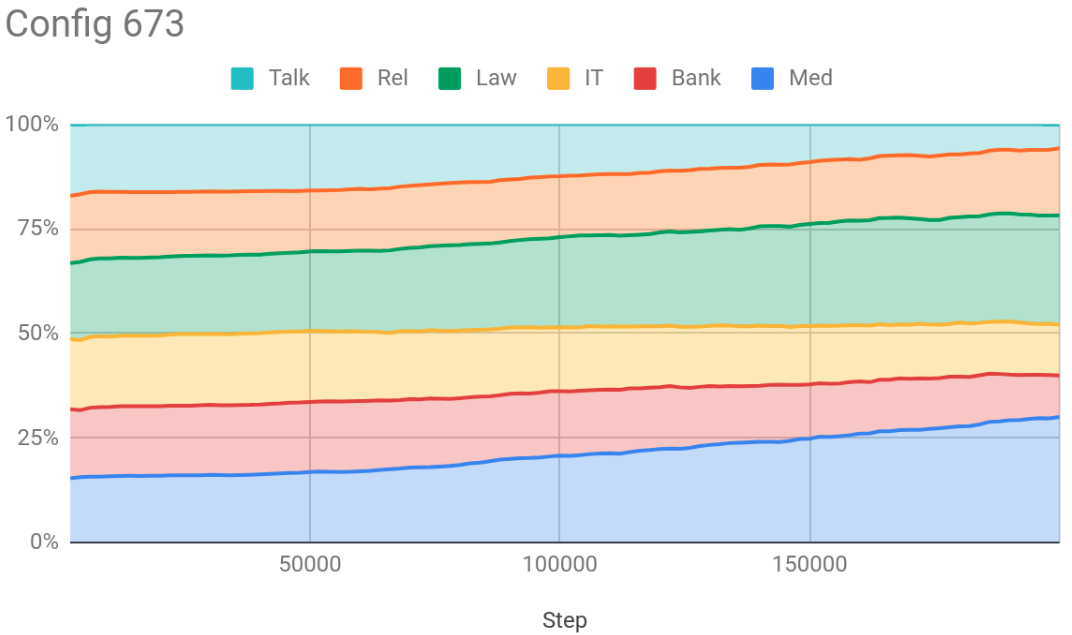
\includegraphics[width=.8\linewidth]{config673.png}  
  \caption{Config 673}
  \label{fig:673}
\end{subfigure}
\caption{Sampling distribution}
\label{fig:sampling}
\end{figure*}

\subsection{Stabilizing the sampler \label{ssec:sampler}}

To stabilize the sampler, we consider two alternatives. The first one is to replace the softmax function, yielding the following updates:\fyTodo{List options}
\begin{align*}
\psi_d = \frac{\psi_d + \eta * R_d}{ 1 + \eta \displaystyle{\mathop{\sum}_{j=1}^{n_d}} R_j},
\end{align*}
where $\eta$ controls the learning rate of $\psi$.

The second one simply adds an entropy constraint which ensures that the entropy of the domain distribution is always greater than a predefined value $\alpha$.\fyTodo{Explain the math}

\subsection{Our version}

\fyTodo{Refaire table 3 + (unsupervised domain in source= classification) + new domain}


\section{Related Work \label{sec:related}}
1. DA
2. Multi-DA
3. Dynamic Data Selection and Curriculum learning

\cite{Wang17instance} uses dynamic weighting (for sentences and domains) for DA.

\cite{Wang20learning-multi} adapts curriculum learning \cite{BengioXX} for multi-domain adaptation, where an optimal instance weighting scheme is found using Bayesian optimization techniques.

Also \cite{Saunders19adaptive}.

\section{Conclusion and outlook \label{sec:discussion}}
\section*{Acknowledgments}
\bibliographystyle{acl_natbib}
\bibliography{multidomain}
%\appendix
\end{document}

Multi-domain learning, as defined in \citet{Dredze08online} further assumes that domain tags are also available in testing; the implication being that the test distribution is also as a mixture of several domains, making the problem distinct from mere domain adaption. A multi-domain learner is then expected to use these tags effectively \cite{Joshi12multidomain} when computing the combined translation function $h(x,d)$, and to perform well in all domains \cite{Finkel09hierarchical}. This setting is closely related to the multi-source adaptation problem formalized in \cite{Mansour09domainadaptation,Mansour09multiple,Hoffman18algorithms}.

This definition seems to be the most accepted view of a multi-domain MT\footnote{An exception is \citep{Farajian17multidomain}, where test translations rely on similarity scores between test and train sentences, rather than on domain labels.} and one that we also adopt here. In the absence of further specification, the naive answer to the MD setting should be to estimate one translation function $\hat{h}_d(x)$ separately for each domain, then to translate using $\hat{h}(x,d) = \sum_{d'} h_{d'}(x) \indic{d' = d}$, where $\indic{x}$ is the indicator function.

Given an objective mixture over test distribution $\lambda^{t}_{d}$,$d\in[1,\dots,K]$ and a mixture of training data $\lambda^{s}_{d}$, the Multi-domain training course is determined by the below algorithm \ref{alg:mdmt}. The training mixture can be constant or changing through time. Optimizing the training mixture is an interesting problem that we would like to address in the paper.

\begin{algorithm}[H]
\caption{Multi-domain Training} \label{alg:mdmt}
\label{alg:multidomain}
\begin{algorithmic}[1]
\REQUIRE {
\begin{itemize}
	\item Corpora $C^d, d\in [1,..,K]$ for $K$ domains equipped by an empirical distribution $D_d(x,y)$
	\item Dev sets $Dev^d, d\in [1,..,K]$ for $K$ domains.
	\item Testing mixture weights in the final evaluation $\lambda^t_d, d\in [1,..,K]$
	\item Batch size $B$.
	\item Temporal Data Selection Distribution(T-DSD)$$P_{\system{T-DSD}}(t)(x,y)=\sum_{d}\lambda^s_d(t)D_d(x,y)$$
	\item $Eval\_scores = []$
	\item $Early\_stopping$ criterion.
\end{itemize}}
\REPEAT 
\STATE{Iteration t.}
\STATE{Randomly pick $d \in [1,..,K]$ w.r.t  $[\lambda^s_1 \dots \lambda^s_K](t)$.}
\STATE{Sample $B$ sentences from $C^d$ with empirical distribution $D_d(x,y)$.}
\STATE{Update model by applying SGD computed from $B$ sampled sentences.}
\IF{$t \equiv 0 \mod{eval\_step}$}
	\STATE{Evaluate current model with $K$ dev sets. $S^t_d$ is the performance at iteration $t$ on domain $d$.}
	\STATE{Report weighted score using testing mixture weights $\lambda^t_d, d\in [1,..,K]$. $$eval(t) = \displaystyle{\mathop{\sum}_d \lambda^t_d S^t_d}$$}
	\STATE{$Eval\_scores.append(eval(t))$.}
\ENDIF
\IF{$Early\_stopping(Eval\_scores)$}
	\STATE{Stop training loop.}
\ENDIF
\UNTIL{convergence}
\end{algorithmic}
\end{algorithm}

